% !TeX spellcheck = en_US
% !TeX root = ../Tom_Sandmann-master_thesis
\section{Matching the templates} \label{sec: Matching the templates}
Using the method as described in \Cref{algo: determining offsets} of \Cref{sec: Determining the offsets} to determine the offsets, we applied the OTA to the {\fourq} hardware design using the SAKURA-G board.
For the very first iteration, the target trace of the relevant doubling operation together with the corresponding template traces can be seen in \Cref{fig: OTA first iteration target example} and \Cref{fig: OTA first iteration templates example} respectively.
An overlap of the template traces can be seen in \Cref{fig: OTA first iteration template traces overlap}.
All of these traces are captured with a sampling rate of 1GSa/s without any bandwidth or noise filter applied.
The signal coupling of the channels was set to $\mathrm{DC}50\ohm$.
The operation speed of the {\fourq} design was set to 1.5MHz (which is the default speed).
Due to the Nyquist-Shannon sampling theorem, we need to capture a power trace at a sample rate that is at least twice the bandwidth of the input signal. 
In addition, it may be preferable to use a sample rate that is (at least) 10 times the acquisition bandwidth, such that fast signal rise times are oversampled in order to make them consistent with the oscilloscope bandwidth \cite{waverunner6manual}.
This justifies our acquisition rate of 1GSa/s.
%
\begin{figure}
	\centering
	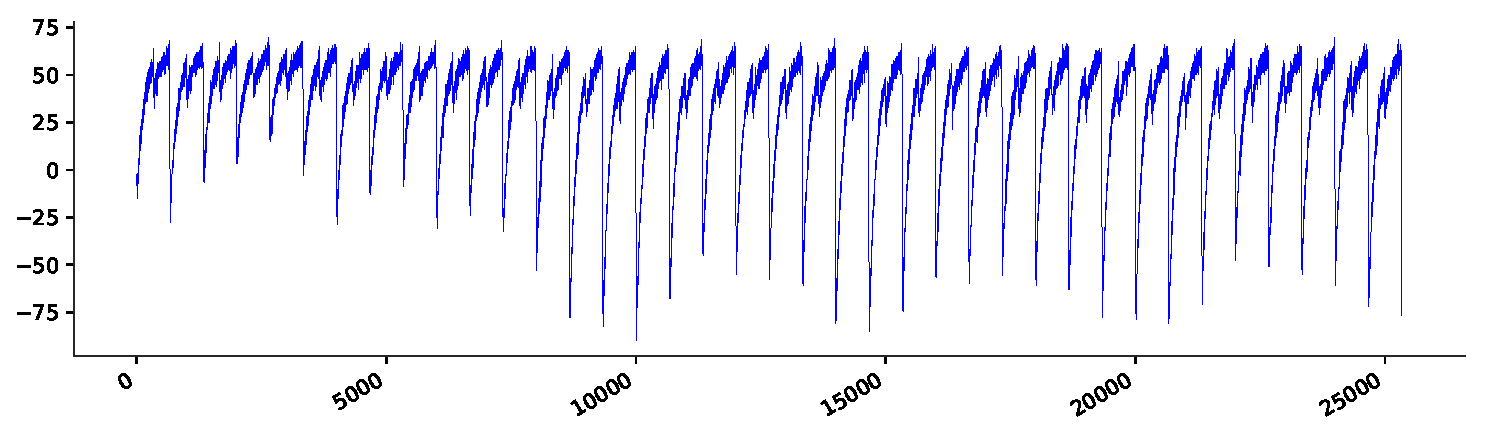
\includegraphics[scale=0.6]{traces/first_doubling/target_trace_dbl_oper_d64}
	\captionof{figure}{Target trace of the first doubling, which is produced using the value $d_{64} = 7$ with the base point and scalar as listed in \Cref{App sec: example template traces} in \Cref{Appendix}.}
	\label{fig: OTA first iteration target example}
\end{figure}
%
\begin{figure}
	\centering
	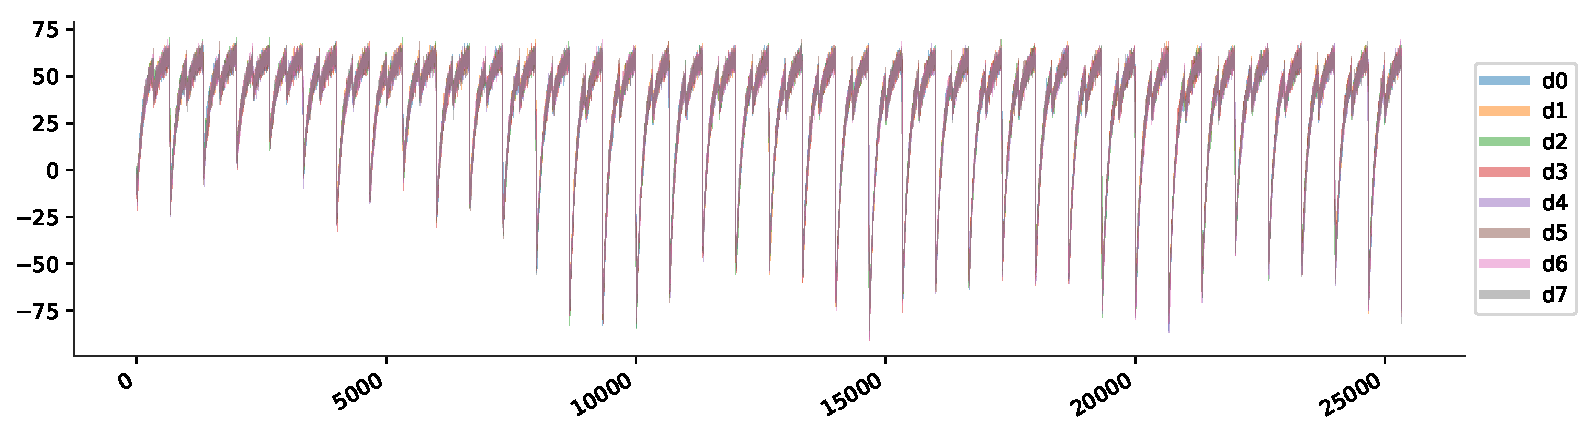
\includegraphics[scale=0.59]{traces/first_doubling/template_traces_overlap_d64}
	\captionof{figure}{An overlap of all the template traces shown in \Cref{App sec: example template traces}.}
	\label{fig: OTA first iteration template traces overlap}
\end{figure}
%
Without even looking at the correlation results, we can immediately see that the template traces are almost identical. 
After viewing the traces in Inspector SCA (a software product developed by Riscure), we can see that there are very small differences between these template traces.
The similarity among the template traces is also reflected in the correlation values obtained after correlating the templates with each other.
These correlation values are at least 99\%.

After correlating the template traces with the target trace using the Pearson correlation coefficient while attacking the first 5 digit-columns (i.e. the first 5 iterations of the OTA), we again observed that all of the correlation values were close to 99\%. 
Instead of only using the doubling operation, we also made use of the fact that we can use the addition operation to have two `operations of reference' instead of one.
Making use of this approach slightly decreased the correlation values.
However, the results were similar to the results observed when \emph{only} making use of the doubling operation.
We decided to research which part of the frequency of the target trace contained the expected leakage.
After applying FFT to the target trace, we found out that the interesting samples were in the higher frequencies of the trace.
This was verified by making use of a low-pass filter with a cut-off frequency of 81MHz.
If the interesting frequencies of a trace are filtered out, the traces will even look more similar, which will result in higher correlation values in the template-matching phase.
This is also exactly what we observed in the correlation values after we applied the aforementioned low-pass filter.
Therefore, we decided not to use this low-pass filter in the remaining experiments we conducted.

\subsection{Bandwidth filter comparison}
As the template-matching results are so close to each other, we decided to attack the first 5 digit-columns (i.e $d_{64}$ up to $d_{60}$) for the same target trace.
Each attack was performed 20 times with different bandwidth filters.
The reason for conducting this experiment is to get more insight in which settings of the oscilloscope are the most promising despite the high similarity among the template traces.
By performing the OTA 20 times using the same settings, we wanted to account for coincidences with respect to the ranking of the template that is expected to have the highest correlation value.
Results of the rankings for the correct template in attacking the first 5 digit-columns can be seen in \Cref{tbl: first 5 digit-columns bandwidth limit comparison}.
%
\begin{table}
	\centering
	%
	\subfloat[][Full.]{
		%	
		\begin{tabular}{*4c}
			\toprule
			& \bm{$\tilde{x}$} &  \bm{$\mu$} & \bm{$\sigma$}\\
			\midrule
				$d_{64}$ & 3.5 &  4.2 & 2.46 \\
				$d_{63}$ & 5.0 & 4.8  & 1.60  \\
				$d_{62}$ & 2.0 & 1.55 & 0.50 \\
				$d_{61}$ & 9.0 & 8.2  & 3.67 \\
				$d_{60}$ & 2.0 & 1.85 & 0.65 \\
			\bottomrule
		\end{tabular}
		%
		\label{tbl: first 5 digit-columns bandwidth full}
	}
	%	
	\vfill
	%
	\subfloat[][200MHz.]{
		%
		\begin{tabular}{*4c}
			\toprule
			& \bm{$\tilde{x}$} &  \bm{$\mu$} & \bm{$\sigma$}\\
			\midrule
			$d_{64}$ & 4.0 & 4.2 & 2.23\\
			$d_{63}$ & 5.5 & 4.55 & 2.18 \\
			$d_{62}$ & 1.5 & 1.5 & 0.50 \\
			$d_{61}$ & 5.5 & 6.4 & 3.83\\
			$d_{60}$ & 1.0 & 1.45 & 0.50\\
			\bottomrule
		\end{tabular}
		%
		\label{tbl: first 5 digit-columns bandwidth 200MHz}
	}
	\hspace{1cm}
	%
	\subfloat[][20MHz.]{
		%
		\begin{tabular}{*4c}
			\toprule
			& \bm{$\tilde{x}$} &  \bm{$\mu$} & \bm{$\sigma$}\\
			\midrule
			$d_{64}$ & 2.0 & 3.4 & 2.44\\
			$d_{63}$ & 4.0 & 3.85 & 1.65\\
			$d_{62}$ & 2.0 & 1.6 & 0.49\\
			$d_{61}$ & 11.5 & 10.5 & 3.61\\
			$d_{60}$ & 1.0 & 1.3 & 0.46\\
			\bottomrule
		\end{tabular}
		%
		\label{tbl: first 5 digit-columns bandwidth 20MHz}
	}
	\captionof{table}{The median ($\tilde{x}$), mean ($\mu$) and standard deviation ($\sigma$) of the rank of the correct template is shown after attacking the first 5 digit-columns. 
	These values were obtained after applying the OTA 20 times using the same target trace. 
	The number of times the expected template had the highest correlation value is 22, 28, and 31 for \protect\subref{tbl: first 5 digit-columns bandwidth full}, \protect\subref{tbl: first 5 digit-columns bandwidth 200MHz} and \protect\subref{tbl: first 5 digit-columns bandwidth 20MHz} respectively.}
	\label{tbl: first 5 digit-columns bandwidth limit comparison}
\end{table}
%
What is interesting to see is that the mean and median values for the rank of the correct template trace in attacking the digit-columns $d_{62}$ and $d_{60} $ is way lower than for the other digit-columns. 
This applies to each of the tables regardless the bandwidth filter applied.
It could be the case that the corresponding parts of the target trace are less noisy for these particular digit-columns, which causes the correct template to have the highest correlation value more often.
For the other digit-columns, it can be seen that both the mean and the standard deviation of the correct template are worse. 
Across most tables, the mean and standard deviations stay roughly the same. 
The mean value of the rank tends to go down for digit-column $d_{61}$ for a bandwidth limit of 200MHz \protect\subref{tbl: first 5 digit-columns bandwidth 200MHz} compared to the full bandwidth \subref{tbl: first 5 digit-columns bandwidth full}.

Based on the data shown in \Cref{tbl: first 5 digit-columns bandwidth limit comparison}, there seems to be no real difference between any of the bandwidth filters, which is probably due to the minimal differences between all of the correlation values. 
If we launch 20 OTA to attack the first 5 digit-columns, we have to make 100 guesses.
This applies to each of the tables shown in \Cref{tbl: first 5 digit-columns bandwidth limit comparison}.
In each of these guesses, we determine which template matches best with the target trace. 
If we compare this total number of guesses to the number of times we matched the correct templates for each of these tables, we get an indication on how bad the classification performance is: between 22-31\%. 
Despite the minimal differences between the number of templates matched correctly, we did however choose to settle with a bandwidth limit of 20MHz for the remaining experiments we conducted.
The reason for this choice is that this bandwidth limit resulted in the highest number of templates matched correctly.
We also note that this is the same bandwidth limit used in a side-channel attack (i.e. a correlation power analysis) on AES to test the performance of the SAKURA-G board once its development had finished \cite{guntur2014side}.
Besides experimenting with different values for the bandwidth limit (None, 20MHz or 200MHz), we also experimented with different sampling rates (from 500 MSa/s up to 20 GSa/s) and coupling values.
However, the correlation results for each possible configuration remained at least 99\% and gave no observable improvement over any of the other configurations we considered.

The high correlation values observed for each of the template traces are not in line with the results that were obtained in \cite{batina2014online}. 
In their experiments, it was observed that a correct template would give a correlation result that was much higher than a non-matching one (i.e. $\ge$97\% when correlating a matching template compared to 85\% for a non-matching template). 
These pattern-matching values would drop when multiple bits were attacked using a single acquisition (which was due to a stability problem with the power supply in their setup).
The previously mentioned results were however obtained on software devices.
These devices have different power properties compared to hardware devices such as FPGAs, which could make these result not directly applicable to our setup.

\subsection{Template averaging}
In \cite{dugardin2016dismantling} an OTA was launched against PolarSSL on an ARM architecture.
When they used a single (non-averaged) template trace to attack a key bit of the scalar, the correlation values observed for the correct templates were low.
They managed to increase the correlation results of the correct template by capturing a template trace multiple times and averaging these results.
By capturing the same template trace multiple times, one can somewhat account for the noise that is present in each acquired template trace.
The effectiveness of this approach depends on the number of additional template traces captured.
It was shown that the correct template had a correlation of 69\% when using a single template trace, while this number increased to 99.80\% when an average of 100 template traces was used.
In \Cref{tbl: first 5 digit-columns template averaging}, the results for applying this template-averaging technique to {\fourq} can be seen \Cref{tbl: first 5 digit-columns template averaging}.
%
\begin{table}
	\centering
	%
	\subfloat[][20 additional templates.]{
		\begin{tabular}{*4c}
			\toprule
			& \bm{$\tilde{x}$} &  \bm{$\mu$} & \bm{$\sigma$}\\
			\midrule
			$d_{64}$ & 3.0 & 3.3 & 1.79 \\
			$d_{63}$ & 5.0 & 5.3 & 1.62 \\
			$d_{62}$ & 1.0 & 1.4 & 0.49 \\
			$d_{61}$ & 6.5 & 6.2 & 3.06 \\
			$d_{60}$ & 2.0 & 1.6 & 0.49 \\
			\bottomrule
		\end{tabular}
	}
	%	
	\vfill
	%
	\subfloat[][50 additional templates.]{
		\begin{tabular}{*4c}
			\toprule
			& \bm{$\tilde{x}$} &  \bm{$\mu$} & \bm{$\sigma$}\\
			\midrule
			$d_{64}$ & 4.5 & 4.6 & 2.33 \\
			$d_{63}$ & 5.5 & 4.9 & 1.92 \\
			$d_{62}$ & 1.0 & 1.2 & 0.40 \\
			$d_{61}$ & 6.5 & 7.0 & 3.52 \\
			$d_{60}$ & 2.0 & 1.6 & 0.49 \\
			\bottomrule
		\end{tabular}
	}
	%	
	\hspace{1cm}
	%
	\subfloat[][100 additional templates.]{
		\begin{tabular}{*4c}
			\toprule
			& \bm{$\tilde{x}$} &  \bm{$\mu$} & \bm{$\sigma$}\\
			\midrule
			$d_{64}$ & 5.0 & 4.1 & 2.47\\
			$d_{63}$ & 4.0  & 3.6 & 1.47 \\
			$d_{62}$ & 1.0 & 1.4 & 0.49 \\
			$d_{61}$ & 6.0 & 6.3 & 3.63 \\
			$d_{60}$ & 2.0 & 1.6 & 0.49 \\
			\bottomrule
		\end{tabular}
	}	
	\captionof{table}{For each attack on the first 5 digit-columns, the median ($\tilde{x}$), mean ($\mu$) and the standard deviation ($\sigma$) of the rank of the correct template is shown when a bandwidth limit of 20MHz is used.
	The indicated number of additional traces (20, 50 or 100) are used to average the acquisition of a single template trace. Each OTA is performed 10 times.}
	\label{tbl: first 5 digit-columns template averaging}
\end{table}
%
As expected, the correlation values become higher once the number of additional template traces increases.
However, classification of the correct template is still far from optimal.
It is almost like throwing a dice to determine the rank of the correct template.
This is very clear if we look at the standard deviation of the rank of the expected template for both \Cref{tbl: first 5 digit-columns bandwidth limit comparison} and \Cref{tbl: first 5 digit-columns template averaging}. 
These results were obtained by making use of the same target trace (which would resemble a real-world scenario).
It could be the case that the attacked digit-columns at which the standard deviation is very high, the corresponding part of the target trace contains more noise than normal.
But due to the non-distinctiveness of the correct template trace, this reasoning remains speculation.
We also applied the averaging technique to the target trace itself (which does not represent a real-world scenario), but this did not yield any results that were more interesting than the usage of one (non-averaged) target trace.

\subsection{Preprocessing the traces}
As we can read in \Cref{subsec: template attacks preprocessing the traces} in \Cref{chp: Side Channel Attacks}, there are some preprocessing steps that we can take into account to improve template matching.
Also a method for selecting the most interesting points in a trace was applied (as described in \Cref{subsec: Making the attack more practical}).
These methods did however not yield improved results.
Besides that, we also made use of the built-in noise filter of the oscilloscope.
Digital oscilloscopes often have a sampling rate that is much higher than required.
This is called oversampling, and can be used to filter the digitized signal to either increase the effective resolution or to remove unwanted noise.
This method is called Enhanced Resolution (ERes).
With the oscilloscope used in our setup, oversampling can be used to increase the vertical resolution.
This is done by making use of moving-average filter \cite{waverunner6manual}.
Application of this particular filter did not gave any observable improvement, as the classification performance was almost identical as observed when applying the techniques discussed before.
Similarly, no improvements were observed with different sampling rates or coupling values of the channel used to capture the template/target trace.

% use Good article on impendance
% https://hackaday.com/2015/07/29/say-it-with-me-input-impedance/